\documentclass[spanish,12pt, a4paper,twoside]{paper}

\let\oldsection\section
\def\section{\cleardoublepage\oldsection}

\usepackage{afterpage}


\newcommand\blankpage{%
\null
\thispagestyle{empty}%
\addtocounter{page}{-1}%
\newpage}

\usepackage[textwidth=15cm, textheight=22.5cm, top=0.5cm, bottom=3.5cm,left= 3cm,right=3cm]{geometry}


\usepackage[spanish]{babel}
%\usepackage[applemac]{inputenc} 
%POR DEFECTO SE ESTa USANDO EL PAQUETE PARA RECONOCER ACENTOS DE MAC, EN CASO DE USAR WINDOWS COMO SISTEMA OPERATIVO ELIMINAR LA LaNEA ANTERIOR E INTRODUCIR LA SIGUIENTE

\usepackage[utf8]{inputenc}

\usepackage{graphicx}
\usepackage{graphics}
\usepackage{amsmath,amssymb}
\usepackage{float}
\usepackage{placeins}
\usepackage{changepage}
\usepackage{subcaption}
\usepackage{algorithm}
\usepackage{multirow}
\usepackage{ragged2e}
\usepackage{enumitem}
\usepackage{mathptmx}



\begin{document}
%\maketitle
%\thispagestyle{empty}
\begin{titlepage}

\newcommand{\HRule}{\rule{\linewidth}{0.5mm}} % Defines a new command for the horizontal lines, change thickness here

\renewcommand{\baselinestretch}{1.5}

\center % Center everything on the page
\vspace*{5pt}
\textsc{\huge Universidad Rey Juan Carlos }
\\[2cm]

% HEADING SECTIONS
%
\includegraphics[width=2.25cm]{recursos/logoFi.png}

\includegraphics[width=6cm]{recursos/escudo_urjc}
\\[2cm]





% TITLE SECTION
\HRule \\[0.4cm]
{ \huge \bfseries Memoria de Prácticas}\\[0.4cm] % Title of your document
\HRule \\[2.5cm]

\textsc{\Large Máster Universitario En Formación del Profesorado de Ed.Secundaria, Bachillerato, FP e Idiomas }\\[0.7cm]
\textsc{ Especialidad en Informática y Tecnología }\\[1cm]

% AUTHOR SECTION
\begin{flushright}
\large
AUTOR: Abel de Andrés Gómez\\
CENTRO: Escuela Politécnica Giner\linebreak
\end{flushright}

\vspace{1cm}

% DATE SECTION
{ {2019}}\\[3cm]
% LOGO SECTION

\vfill % Fill the rest of the page with whitespace

\end{titlepage}

\newgeometry{textwidth=15cm, textheight=22.5cm, top=3.5cm, bottom=3.5cm,left= 3cm,right=3cm}

%Separacion de los listados
\setlist[itemize,2]{topsep=0mm}
\setlist[itemize]{itemsep=0mm}

\afterpage{\blankpage}
\pagenumbering{roman}
\setlength{\parskip}{8pt}

% ÍNDICE
\tableofcontents % indice de contenidos


% CAPaTULOS DEL TRABAJO FIN DE MaSTER
\newpage
\pagenumbering{arabic} 



\section{INTRODUCCIÓN} % 1-2 paginas
%En este primer apartado de la memoria de prácticas, se va a proceder a realizar una descripción sobre la estancia personal en el centro de prácticas.

En este primer apartado de la memoria de prácticas, se va a proceder a realizar una breve descripción sobre las expectativas personales, la contextualización del centro y la documentación que se ha manejado.

En primer lugar, es necesario destacar que es la primera vez que he tenido la ocasión de ejercer como docente, por tanto, existían unas expectativas que partían de la base de aprender como ejercer la docencia y eliminar cualquier posible miedo que se pueda tener en el aula. Por tanto, durante todas las clases en las que he asistido, he tenido una actitud de observación. Intentando aprender sobre situaciones en el aula puesto que en un futuro no me encontrare acompañado por ningún docente. También he tenido una actitud de interacción con los alumnos lo máximo posible, siendo una persona extrovertida. De esta forma he conseguido eliminar cualquier miedo que pueda existir.

Por otro lado, me he dado cuenta que la docencia requiere una serie de horas que el docente necesita para preparar las sesiones que impartirá en clase. De esta forma, he comprobado también que los niveles superiores son más complejos que los inferiores, puesto que requiere un mayor preparamiento de las sesiones a impartir. Sin embargo, también he comprobado que el temario no es complejo, por lo que los miedos a explicar el contenido de una asignatura han remitido.

En cuanto al desarrollo profesional, puedo destacar el aprendizaje de aptitudes y conocimientos. Por tanto, no solo he aprendido a educar y enseñar a terceros, sino que también he recuperado conocimientos ya olvidados. Entre conocimientos muy concretos puedo destacar aquellos relacionados con las redes de computadoras. De esta forma, también me he dado cuenta que las practicas me han ayudado a obtener conocimientos, pero lo importante y lo que mejor he asimilado han sido las formas de actuar ante diversas situaciones.

El primer día de contacto con el tutor me enseño el centro, indicándome los lugares e instalaciones que este dispone. Me di cuenta que, para ser un centro pequeño en dimensiones, tiene un gran número de alumnos matriculados, rondando los 500. Por tanto, a simple vista se puede observar una gran gestión del centro.

Para situarnos en contexto, las practicas se han desarrollado en el centro Politécnica Giner, este centro ofrece una serie de enseñanzas en distintos niveles.
Respecto a las enseñanzas que imparte son las siguientes:
\begin{itemize}
\item En Formación Básica Profesional:
\begin{itemize}
\item Servicios Administrativos
\item Informática y Comunicaciones
\item Servicios Comerciales
\item Peluquería y Estética
\end{itemize}
\item En Grado Medio
\begin{itemize}
\item Actividades Comerciales
\item Cuidados Aux. de Enfermería
\item Estética y Belleza
\item Peluquería y Cosmética Capilar
\item Sistemas Microinformáticos y Redes
\item Gestión Administrativa
\end{itemize}
\item En Grado Superior
\begin{itemize}
\item Educación Infantil
\end{itemize}
\item Educación Secundaria Personas Adultas
\end{itemize}

Durante estas prácticas, he asistido a la impartición de asignaturas en el ámbito de la informática. Concretamente, he asistido a la docencia de asignaturas relativas a la enseñanza de \textit{Informática y Comunicaciones} de Formación Básica Profesional y \textit{Sistemas Microinformáticos y Redes} de Grado Medio.

El centro educativo se encuentra en el distrito de "Latina", concretamente en el barrio de Campamento, barrio mayormente de población obrera. La titularidad del centro es Privado/Concertado, sin embargo, los niveles en los que he asistido son públicos. 

Teniendo en cuenta la situación geográfica del centro y el nivel educativo en el que he asistido, el rechazo escolar es una situación a la que los alumnos están predispuestos. 

Centrándonos en la organización del centro, podemos destacar que existe un equipo directivo formado por 3 personas distintas que asumen el cargo de director, jefe de estudios y secretario. Por otro lado, existe un coordinador por cada uno de los departamentos existentes, existiendo un departamento por aproximadamente cada enseñanza de la oferta educativa y un departamento de orientación y otro de biblioteca.

El centro tiene un total de 42 profesores, siendo 32 de ellos titulares, 10 adjuntos, 31 fijos y 11 temporales. También existe una persona encargada de la administración y 3 personas responsables de la limpieza del centro.

Por último, respecto a la documentación que se ha manejado, ha sido la siguiente:
\begin{itemize}
\item \textbf{Programación General Anual (P.G.A)}. Se ha revisado la programación de algunas de las asignaturas de Formación Profesional Básica y de Grado Medio. También se ha revisado las unidades de dichas asignaturas y el criterio de evaluación.
\item \textbf{Proyecto Curricular de Centro (P.C.C)}. Concretamente se ha revisado el relacionado con el Grado Medio de \textit{Sistemas Microinformático y Redes}, que es al que he asistido. En este documento aparecen todas las asignaturas que se imparten durante los dos cursos escolares que dura el Grado. Se indica también el número de horas, objetivos y contenido de cada asignatura y las unidades de competencia generales
\item \textbf{Memoria Anual del Centro}. 
\begin{itemize}
\item Se muestra el personal y los órganos de dirección y gestión del centro. Distingue entre equipo directivo, consejo escolar y departamentos.
\item Contiene el analisis y los resultados academicos del curso.
\item Se indican los programas, planes y proyectos desarrollados.
\item Se muestra los grados de consecución de objetivos de la P.G.A.
\end{itemize}
\item \textbf{Proyecto Educativo de Centro (P.E.C)}. Se ha revisado este documento para obtener algunas ideas sobre el entorno de la Escuela Politécnica Giner y su contexto. En este documento se encuentra nuevamente la organización y gestión del centro y su personal. Se muestra también su ideario concertado, laico y plural. También se muestran los objetivos educativos de la escuela. Por último, también contiene las normas de organización, funcionamiento y convivencia.
\end{itemize}
%El buen profesor. La milla verde

\section{PROGRAMACIÓN} % 2-3 paginas

En este apartado se va a realizar una breve descripción sobre la programación de la asignatura de \textit{Redes Locales}. A pesar de haber impartido clases en varias asignaturas y varios niveles educativos, se va a realizar la descripción de esta asignatura puesto que será sobre la que se va a realizar la unidad didáctica. 

La asignatura de \textit{Redes Locales} se imparte en el Ciclo Formativo de Grado Medio, en la familia profesional de la Informática y Comunicaciones y a su vez se encuentra en la especialidad de Sistema Microinformático y Redes.

En la Programación General Anual (P.G.A) de la asignatura de \textit{Redes Locales} se recogen una serie de características sobre la asignatura, como por ejemplo las competencias generales del grado, la relación de cualificaciones y unidades de competencia, los objetivos generales del módulo, la temporalización de las tareas, las unidades de trabajo (con sus objetivos, contenidos y criterios de evaluación), la metodología, las actividades, los recursos didácticos, etc. Esta P.G.A debe actualizarse cada curso escolar.

Centrándonos en la temporalización, la P.G.A comenta que el orden de los contenidos es orientativo y a su vez, estos deben realizarse mediante criterios racionales y pedagógicos.

Los criterios que se tienen en cuenta para la secuenciación de dichos contenidos son los siguientes:
\begin{itemize}
\item Adecuación al desarrollo evolutivo del alumnado.
\item Adaptación de los contenidos a los conocimientos previos del alumnado.
\item Continuidad y progresión en los contenidos.
\item Equilibrio entre las secuencias de conceptos, objetivos y capacidades.
\item Interrelación entre contenidos.
\end{itemize}

A continuacion se va a mostrar la estructura y la relación ordenada de las unidades de trabajo junto con el número de horas lectivas.
\begin{itemize}
\item \textbf{Primera Evaluación}
\begin{itemize}
\item \textbf{Unidad 1.} Sistemas de comunicación y redes \textit{(15 horas lectivas)}.
\item \textbf{Unidad 2.} Arquitectura y redes \textit{(30 horas lectivas)}.
\item \textbf{Unidad 3.} Caracterización de redes de área local \textit{(35 horas lectivas)}.
\end{itemize}
\item \textbf{Segunda Evaluación}
\begin{itemize}
\item \textbf{Unidad 4.} Identificación de elementos y espacios de una red local \textit{(35 horas lectivas)}.
\item \textbf{Unidad 5.} Instalación y configuración de los equipos de red \textit{(40 horas lectivas)}.
\end{itemize}
\item \textbf{Tercera Evaluación}
\begin{itemize}
\item \textbf{Unidad 6.} Interconexión de equipos en red de área local \textit{(45 horas lectivas)}.
\item \textbf{Unidad 7.} Resolución de incidencias de una red de área local \textit{(15 horas lectivas)}.
\item \textbf{Unidad 8.} Cumplimiento de las normas de prevención de riesgos laborales y protección medioambiental \textit{(5 horas lectivas)}.
\end{itemize}
\end{itemize}

El resto de horas lectivas, hasta 230 que componen el módulo de \textit{Redes Locales} se van a dedicar a realizar ejercicios de evaluación.

La unidad fundamental en la que nos centraremos va a ser la \textit{Unidad 5. Instalación y configuración de los equipos de red}. Esta unidad va a servir de base para el desarrollo del siguiente punto de esta memoria.

Algunos de los \textbf{objetivos} a destacar de la asignatura son los siguientes:
\begin{itemize}
\item Conocer los medios de direccionamiento físico de los equipos que forman la red.
\item Estudiar las formas de direccionar equipos en internet mediante la dirección IP.
\item Ver como las direcciones IP nos permiten definir subredes dentro de una red.
\item Estudiar el protocolo IP.
\end{itemize}


Para conseguir dichos objetivos, se establece una metodología de enseñanza-aprendizaje, basada en el \textbf{modelo constructivista de aprendizaje} que consiste en relacionar los conocimientos previos y los que se desea que el alumno aprenda. Este modelo integra los principios psicopedagógicos y metodológicos y conduce al diseño de actividades enseñanza-aprendizaje.

Siguiendo este modelo, las clases teóricas se van a alternar con la resolución practica de ejercicios, de forma individual y en grupo. Estos ejercicios prácticos van a servir para fijar y aplicar los conocimientos, resolver las dudas que puedan aparecer y para introducir las técnicas y procedimientos explicados en clase, así como a la utilización de herramientas apropiadas. %De esta forma se potencia la capacidad crítica del alumno, se estimula su curiosidad y se practica técnicas de dialogo y debate para llegar a acuerdos consensuados.

Algunos tipos de \textbf{actividades} que se realizan son las siguientes:
\begin{itemize}
\item \textbf{Actividades de conocimientos previos}. Desarrollo de esquemas o cuestionarios para conocer las ideas, opiniones, aciertos o errores de los alumnos sobre los contenidos que se van a desarrollar.
\item \textbf{Actividades de exposición y debate del trabajo}.Para que los alumnos sean capaces de expresar sus ideas y contenidos adquiridos.
\item \textbf{Actividades de documentacion}. Cada practica que se realice, debe documentarse.
\item \textbf{Actividades de seguimiento}. Por parte del profesor, de los trabajos realizados por los alumnos.
\item \textbf{Actividades de síntesis-resumen}. Para facilitar la relación entre los distintos conocimientos comprendidos y favorecer el enfoque globalizador.
\item \textbf{Actividades de refuerzo y ampliación}. Para los alumnos que no hayan alcanzado los objetivos deseados o para aquellos que los han realizado satisfactoriamente.
\item \textbf{Actividades de grupo}. Se deben utilizar criterios para la formación de grupos, atendiendo a la diversidad de intereses de los alumnos que lo componen, así como las capacidades de los mismos.
\end{itemize}

%Por otro lado, también van a existir \textbf{actividades de recuperación} que se clasificaran del siguiente modo:
%\begin{itemize}
%\item \textbf{Actividades de recuperación para las unidades de trabajo o bloques de unidades}. Cada evaluación se recupera antes de la entrega de notas de esa evaluación, mediante una prueba escrita acompañada de las practicas que no se hayan realizado.
%\item \textbf{Actividades de recuperación de la totalidad del módulo o bien de parte del mismo}. Se van a realizar en el mes de junio, con anterioridad a la evaluación ordinaria del curso.
%\end{itemize}


Los \textbf{recursos} que se van a emplear para realizar las siguientes actividades son:
\begin{itemize}
\item \textbf{Aula Virtual, Moodle}. A través de ella se desarrollan las actividades de debate, foros, encuestas, entrega de tareas y calificación de las mismas.
\item \textbf{Pizarra}. Permite una adecuada visualización de los conceptos expuestos.
\item \textbf{Proyector}. Permite presentar esquemas, gráficos y otros recursos útiles para realizar la explicación de un contenido.
\item \textbf{Libros de texto}. Contiene la información fundamental que el alumno debe aprender.
\item \textbf{Ordenadores}. Permite al alumno documentarse y realizar las actividades prácticas, además permite el trabajo con distintas aplicaciones.
\item \textbf{Etc.}
\end{itemize}

Por último, se va a realizar una breve descripción sobre la \textbf{evaluación de la asignatura}. Dicha evaluación debe cumplir una serie de fines que se encuentran en la P.G.A. Por otro lado, la evaluación continua se divide en tres fases: evaluación inicial, formativa y sumativa; cada fase tendrá unas pretensiones distintas. 

Como procedimiento para la evaluación, se utilizan las pruebas, que sirven para valorar el rendimiento de los alumnos. Dichas pruebas se tendrán en cuenta por cada unidad de trabajo y vendran acompañada por el \textbf{criterio de calificación}. Siendo las pruebas junto con sus criterios de evaluación las siguientes:
\begin{itemize}
\item Asistencia, actitud y participación: \textbf{10\%}
\item Pruebas escritas: \textbf{70\%}
\item Prácticas: \textbf{20\%}
\end{itemize}

Como ya se ha comentado, cada unidad se va a calificar ponderando cada uno de los puntos anteriores que se haya realizado, calificando de 0 a 10 con dos decimales.

En la P.G.A se muestra también la \textbf{convocatoria extraordinaria} (se realizan el mes de junio). Se presentan aquellos alumnos que no hayan logrado evaluación positiva en la convocatoria ordinaria. Esta convocatoria abarca todos los contenidos de la asignatura, y los alumnos que se presenten lo realizaran en su totalidad, ya que la nota sera global del curso. Las practicas se guardan como entregadas durante todo el curso escolar.

Por último, la asignatura establece medidas de atención al alumnado con \textbf{necesidades educativas especiales} (ACNEE). Para estos alumnos se debe realizar caminos de atención a la diversidad como refuerzos educativos, tutorías y adaptaciones curriculares. Las adaptaciones van a ser diferentes en función de la diversidad. Algunas medidas de adecuaciones comunes son:
\begin{itemize}
\item Las tutorías.
\item La dificultad de las actividades se establece gradualmente de menor a mayor dificultad, para que los alumnos encuentren espacios adecuados a sus capacidades.
\item Las actividades de aplicación y los ejercicios propuestos se van a desarrollar en grupos heterogéneos, prestando atención al reparto de tareas y a una asignación de funciones flexible.
\end{itemize}

\section{UNIDAD DIDÁCTICA} %3-5 paginas

En primer lugar, es necesario tener en cuenta que a lo largo de las practicas, no se ha desarrollado una unidad completa, sino que se ha realizado una parte de esta. Sin embargo, se ha intentado realizar actividades en las distintas asignaturas con el objetivo de abarcar las máximas etapas y metodologías en el proceso de enseñanza.

Durante el periodo de prácticas se ha realizado una actividad de supervisión a lo largo de todas las asignaturas ejerciendo una función de docente. Se han resuelto las dudas de los alumnos a lo largo de la realización de las practicas sugeridas por el docente. Concretamente se ha supervisado las asignaturas de \textit{Servicios en Red}, \textit{Sistemas operativos en red} y \textit{Sistemas operativos monopuesto} (todas estas asignaturas se imparten en primero y segundo de grado medio). Esto se debe a que estas asignaturas son totalmente prácticas, donde los alumnos deben realizar instalaciones y configuraciones sobre los sistemas Windows y Linux. De esta forma, los alumnos deben seguir un guion realizado por el docente con el objetivo de resolver las practicas. Sin embargo, muchas veces los alumnos cometen errores en la instalación y la configuración y hace que estos no puedan continuar con la práctica y, por lo tanto, requieren atención, una persona que les ayude a resolver los problemas prácticos.

En segundo lugar, se han realizado actividades mediante Kahoot para los alumnos de Grado Básico principalmente, puesto que la gamificación en este nivel es fundamental, ya que como se ha comentado con anterioridad, los alumnos tienden al rechazo escolar. De esta forma, se ha realizado actividades con Kahoot en asignaturas como \textit{Montaje y Mantenimiento de sistemas informáticos}, \textit{Equipos eléctricos y electrónicos} y \textit{Operaciones Auxiliares para la configuración de equipos}. Con esta herramienta de gamificacion, se pretende reforzar los conocimientos de los alumnos de cara a los exámenes que tienen que realizar. Por tanto, ha sido necesario revisar el contenido de las unidades para poder formular las preguntas y las respuestas.

En la asignatura de \textit{Montaje y Mantenimiento de sistemas informáticos} además de realizar el Kahoot sobre el tema de dispositivos de almacenamiento, se ha realizado en varias ocasiones un juego en el que el docente tenía que escribir en papeles ciertos periféricos o conceptos que quisiera. Posteriormente se crean grupos de alumnos, cada grupo tiene un representante. Una vez que están los grupos creados, entonces se distribuían los papeles a cada representante. Estos representantes tenían que describir mediante sinónimos o mediante contexto los conceptos o los periféricos que aparecían en los papeles. Siendo, por tanto, una idea sacada del famoso juego de mesa \textit{"Pictionary"}.

Esta asignatura tiene una parte práctica importante, en la que los alumnos deben ser capaces de desmontar periféricos completamente y montarlos nuevamente sin que estos hayan perdido funcionalidad. Por tanto, ha sido necesaria también una labor de supervisión y resolución de dudas a los alumnos. Entre algunos periféricos que tienen que desmontar son el disco duro, la unidad óptica y el teclado.

\begin{figure}
\centering
\begin{subfigure}[b]{0.3\textwidth}
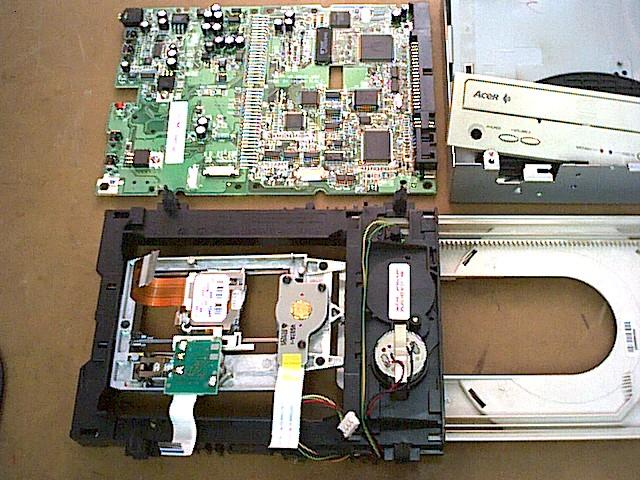
\includegraphics[width=\textwidth]{recursos/cdrom2.jpg}
\caption{Unidad óptica}
\end{subfigure}
~ %add desired spacing between images, e. g. ~, \quad, \qquad, \hfill etc. 
%(or a blank line to force the subfigure onto a new line)
\begin{subfigure}[b]{0.3\textwidth}

\includegraphics[width=\textwidth]{recursos/disco-duro.jpg}
\caption{Disco duro}
\end{subfigure}
\begin{subfigure}[b]{0.3\textwidth}
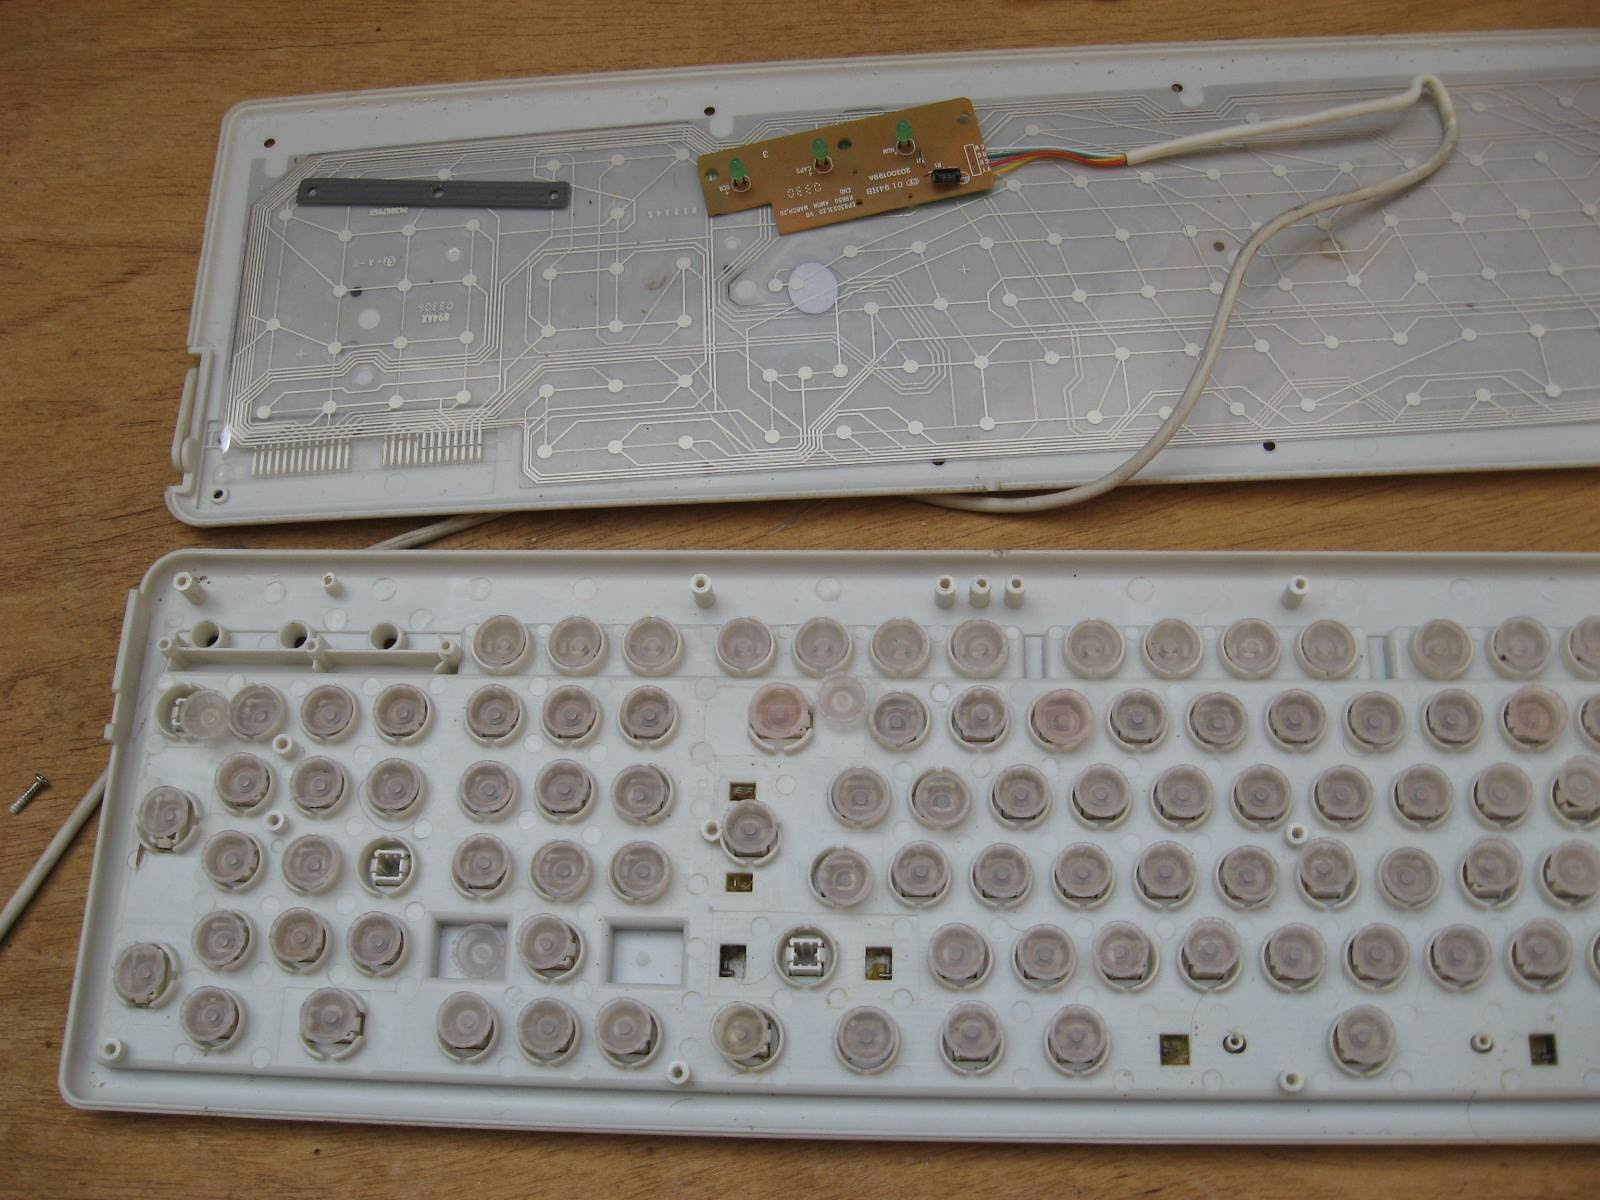
\includegraphics[width=\textwidth]{recursos/teclado.jpg}
\caption{Teclado}
\end{subfigure}
~ %add desired spacing between images, e. g. ~, \quad, \qquad, \hfill etc. 
%(or a blank line to force the subfigure onto a new line)
\caption{Desmontando componentes}
\end{figure}
\FloatBarrier

En las asignaturas de \textit{Equipos eléctricos y electrónicos} y \textit{Operaciones Auxiliares para la configuración de equipos} también se ha realizado otra serie de juegos para que los alumnos consoliden los conocimientos. Entre las actividades realizadas para este fin, se ha utilizado una técnica de preguntas y respuestas entre alumnos siguiendo la filosofía del \textit{Trivial}. En este juego, los alumnos (en grupos o individualmente) tienen que buscar en el tema del libro correspondiente preguntas que otros alumnos deben contestar. Para la búsqueda de estas preguntas los alumnos disponen de 30 segundos. Los alumnos que responden a las preguntas posteriormente deben formular otras nuevas del mismo tema y así, sucesivamente. Esta técnica hace que los alumnos que tengan dificultades para estudiar deban memorizar la pregunta ya que durante la formulación no se permite el uso del libro. Por otro lado, los alumnos que responden, deben también memorizarse la respuesta. Pasado el tiempo límite, si los alumnos no son capaces de responder, automáticamente se salta el turno a otro grupo de alumnos.

\begin{figure}[h]
\centering
\begin{subfigure}[b]{0.3\textwidth}

\includegraphics[width=\textwidth]{recursos/kahoot.png}
\caption{Kahoot!}
\end{subfigure}
\begin{subfigure}[b]{0.3\textwidth}

\includegraphics[width=\textwidth]{recursos/pictionary-1200}
\caption{Pictionary}
\end{subfigure}
\begin{subfigure}[b]{0.3\textwidth}

\includegraphics[width=\textwidth]{recursos/trivial.jpg}
\caption{Trivial}
\end{subfigure}
\caption{Herramientas Gamificación}
\end{figure}


En la asignatura de \textit{Equipos eléctricos y electrónicos}, también tuve la oportunidad de prepararme una sesión en la cual, tenía que ayudar al docente encargado a supervisar a los alumnos. Estos tenían que realizar circuitos en las placas \textit{"protoboard"}, por tanto, tuve que recordar conceptos como las bandas de las resistencias, el uso del transistor, como conectar cada componente en la placa, la dirección de la corriente en estas, etc. Esta labor es delicada si no se dedica tiempo en recordar estos conceptos, puesto que, si usas componentes eléctricos, tienes que tener en cuenta ciertos aspectos para evitar que dichos componentes a la hora de conectarse se puedan romper.


Por otro lado, como parte de la unidad didáctica, se ha realizado también una práctica para los alumnos de la asignatura de \textit{Seguridad Informática de segundo} de Grado Medio. Esta práctica consiste en la realización de un análisis de paquetes utilizando la herramienta de Wireshark. Para ello, se ha realizado un pequeño manual de instalación y configuración de este Software, además, se ha realizado unas instrucciones para que los alumnos sean capaces de seguir el manual. No obstante, esta práctica se ha realizado paso a paso en el aula, de esta forma, los alumnos han podido seguir la explicación. El principal objetivo es el descubrimiento de contraseñas en entornos web inseguros mediante la captura de paquetes. Esta actividad se va a localizar en la \textit{Unidad 5. Redes Seguras}. Los objetivos que se pretenden satisfacer son:
\begin{itemize}
\item Saber a qué factores se debe la vulnerabilidad del software.
\item Distinguir por sus métodos y peligrosidad a los distintos tipos de intrusos informáticos.
\item Alcanzar conocimientos suficientes para controlar la red, poner atención frente a posibles ataques e intrusiones y saber detectarlos.
\item Impedir, en la medida de lo posible, la interceptación de la información.
\end{itemize}


Respecto a la asignatura de \textit{Redes Locales}, en primer lugar y antes de proceder a realizar la unidad didáctica, se ha tenido un previo contacto con los alumnos mediante la corrección de exámenes de la unidad previa, de esta forma, gracias a la ayuda del docente de la asignatura, he aprendido a corregir exámenes, labor que no es tan simple como pueda parecer. Por otro lado, como persona que ha corregido los exámenes, he tenido que estar en la revisión de estos por si algún alumno tenía alguna duda sobre los criterios de evaluación.

Por otro lado, se me ha encargado una parte de la \textit{Unidad 5. Instalación y configuración de los equipos de red}. Los contenidos de esta parte de la unidad se centraban en la parte del direccionamiento IP y el cálculo de subredes. De esta forma, se ha preparado esta parte utilizando 3 sesiones de una hora cada una. De esta forma, se ha realizado una lección magistral en la que se ha enseñado a los alumnos los conceptos básicos de las IP, indicando que existen 5 clases de IPs, que rango abarcan cada tipo y que consecuencias conlleva el uso de unas u otras. Se ha enseñado también que parte de las IPs identifican la red y que parte identifica el host. Para realizar esta sesión, he tomado los apuntes y las diapositivas que el docente me ha proporcionado, indicándome la posibilidad de corrección y actualización de dichos apuntes en caso necesario y bajo una posterior revisión. Al final de esta sesión se ha realizado un pequeño ejemplo en pizarra de lo explicado con anterioridad y se ha encargado la resolución de una hoja con 3 problemas que los alumnos deberán realizar en casa.

En la segunda sesión, se ha corregido el ejercicio que se pidió en la sesión anterior. Obviamente, he tenido que elaborar dicho ejercicio y obtener y comprobar con el docente los resultados que he obtenido, de esta forma garantizábamos que los ejercicios solicitados tienen coherencia y que los resultados son correctos. Esta práctica es algo fundamental, puesto que ofrece mucha seguridad a la hora de realizar dicho ejercicio en pizarra. Debido a que la mayoría de los alumnos no han conseguido terminar el ejercicio completo (ya que no lo comprendían correctamente), se ha dedicado esta sesión a la resolución de este ejercicio paso a paso para que todo el mundo pueda comprenderlo. Una vez se les ha dejado ejercicio a los alumnos, que deberán realizar en casa para corregirlos en la siguiente sesión.

En la tercera sesión, al igual que en la segunda, se ha corregido los ejercicios utilizando la pizarra. Al igual que en la sesión anterior, muchos de los alumnos no han realizado las actividades, por lo tanto, se ha decidido elegir a alguno de ellos (aquellos que se ha considerado que no tienen los conocimientos suficientes). Como es de esperar, estos alumnos no han conseguido resolver los problemas sin ayuda, sin embargo, se ha conseguido que estos hayan obtenido los conocimientos esperados. Para conseguir afianzar los conocimientos relativos a esta parte importante de la asignatura de redes (que tendrán que usar en el futuro), se ha creado una hoja con 10 ejercicios que los alumnos deberán realizar durante la siguiente sesión. Una vez más, se ha encargado a los alumnos que salgan a la pizarra a resolver dichos ejercicios. Con estos ejercicios resueltos, se va a realizar un examen únicamente sobre esta parte.

El docente encargado de la asignatura me ha dejado realizar un pequeño examen valorado en aproximadamente 1,5 puntos de la nota final de la asignatura en la evaluación. Este examen consta de 4 preguntas, en las que se ha evaluado sobre 100, dando 70 puntos a la primera pregunta, 5 puntos a la segunda, otros 5 puntos a la tercera y 20 puntos a la cuarta pregunta, siendo la total puntuación de 100. Se ha considerado utilizar esta puntuación puesto que, a mi parecer, resulta más sencillo trabajar sobre números enteros que sobre decimales. Sobre todo, cuando los problemas son numéricos, y los resultados son exactos y no existe ambigüedad posible. De cualquier forma, no solo se va a tener en cuenta los resultados finales, sino que también se va a evaluar el razonamiento para llegar a estos resultados. 

La experiencia corrigiendo exámenes ha sido optima, los resultados no han sido buenos, ya que solo han aprobado 5 personas de 11 en total. Esto se debe a la falta de estudio y ganas de los alumnos, puesto que dos de las preguntas han sido ejercicios realizados en clase. Los pedí expresamente que observaran su nota y la volvieran a calcular por si había cometido un error. El día de la entrega del examen, realice la corrección en la pizarra, y el docente, subió el ejercicio a la plataforma virtual para que todo el mundo pudiera verlo y realizarlo.

Una vez realizada la corrección, he realizado un ejercicio de direccionamiento IP en el \textit{Packet Tracer}. Este ejercicio trataba de realizar subredes a partir de la IP de una red. El ejercicio lo he realizado a través del equipo del docente, de esta forma los alumnos podían seguir la explicación y realizarlo al mismo tiempo en sus equipos. Una vez acabado, he comprobado que todos los alumnos lo habían realizado, y que las subredes que habían montado realmente funcionan. Esta actividad la han tenido que subir a la plataforma virtual para que el docente la corrigiera, puesto que ha sido el último día de prácticas.

Con estas actividades, concluye lo que ha sido mi unidad didáctica, en la que he tratado de realizar como ya he comentado con anterioridad todas las etapas y actividades que puede realizar un docente. Con esta unidad didáctica además he aprendido cuales eran mis puntos fuertes y débiles con el objetivo de mejorarlos como futuro docente. Como puntos fuertes puedo destacar mi comportamiento extrovertido en el aula, que hace que los alumnos establezcan un vínculo de amistad y que fomente la motivación de estos. Por contra, el punto débil es quizá la explicación en clase, puesto que, aunque las sesiones que he realizado no han estado mal, sí que debo destacar quizá una inseguridad a la hora de realizar la explicación, y, por tanto, algunos de los alumnos tenían dificultad a la hora de comprender dicha explicación. De estos errores e inseguridades, uno como docente debe aprender y ahí está el fundamento de estas prácticas.


\section{CONCLUSIÓN Y VALORACIÓN PERSONAL} %1-2 paginas

A lo largo del desarrollo de las prácticas en el centro docente, he establecido relaciones con distintos profesores que me han aportado muchos conocimientos tanto en el ámbito de ejercer la docencia como a nivel de contenidos, algo de lo que estoy muy agradecido. Como ya he comentado, he descubierto una gran diferencia entre los distintos niveles de alumnos, pues cada nivel tiene alumnos que se encuentran en distintas etapas de la adolescencia. 

Otro aspecto del que me he dado cuenta es que existen ciertos alumnos que causan la inestabilidad total de un grupo en su mayoría. En este aspecto, he tenido la ocasión de observar un par de alumnos que eran capaces de alterar al resto, y, que, en sus ausencias, el grupo permanecía totalmente normal. También se ha visto este mismo efecto con un alumno que tenía una conducta similar al TDAH. Su ausencia producía un mayor rendimiento en los compañeros que le rodeaban.

Ya se ha comentado en la introducción el contexto en el que se sitúa el centro, por lo que en este aspecto incido en la dificultad añadida que tienen los docentes teniendo en cuenta el rechazo escolar de los alumnos. En este sentido, impartir docencia a estos alumnos es algo especial, teniendo sus ventajas y desventajas. Impartir docencia a estos alumnos es complejo y en ello reside el reto. Conseguir atraer a los alumnos en esta situación es difícil, sin embargo, el docente debe dotarse de medios para evitar esta situación. 

En consiguiente si eres una persona muy estricta y exigente con los alumnos, estos no asisten a las clases, por contra, si eres muy permisivo, entonces los alumnos tienen comportamientos inaceptables. Por tanto, es necesario "dar una de cal y otra de arena", expresión bastante usada por los docentes en este nivel educativo. De esta forma, he aplicado esta expresión durante toda mi estancia. 

Por tanto, una persona que aprenda a ser docente, debe situarse totalmente en el contexto en el que se encuentra. Una mala actitud de un alumno no siempre puede ser castigada (teniendo en cuenta las edades con las que se trabaja y la situación de rechazo escolar) puesto que, de ser así, esto puede conllevar al absentismo del alumno. Aquí es donde es necesario que los alumnos no solo te vean como un docente al que muchas veces asimilan como a una persona autoritaria y negativa para ellos, sino como algo más. 

Relacionado con la idea anterior, he aprendido que la docencia es bastante distinta a otros trabajos, puesto que, en el caso de esta profesión, estas tratando o trabajando con alumnos, seres humanos bastante maleables, siendo esta cualidad muy importante a tener en cuenta. Cualquier factor, puede alterar el comportamiento futuro de los alumnos, por tanto, es necesario pensar no solo en la consecuencia instantánea de un acto, sino en las consecuencias futuras de este.

Desde mi punto de vista, dar clase a alumnos de formación profesional tiene la desventaja que no solo enseñas, sino que también la gran mayoría de veces debes educar. También tiene la desventaja que muchas veces parece que los alumnos no retienen la información, son más complicados de motivar y más difícil de enseñar. Sin embargo, tiene una ventaja doblemente añadida, puesto que conseguir que estos tipos de alumnos aprendan algo o tomen una determinada actitud, es mucho más satisfactorio que con alumnos de otros niveles. Personalmente no puedo juzgar sobre que es mejor o que es peor puesto que no he tenido experiencia con otros niveles educativos.

Por último, debo destacar la gran utilidad que tienen estas prácticas, puesto que obtienes una gran cantidad de conocimientos (ya sean relativos al propio acto de docencia como de otras actividades en la labor docente -documentación, reuniones con padres y otros docentes, etc-), y no solo eso, sino que también te metes en el contexto educativo en el aula. De esta forma, como ya he comentado, eres capaz de ver tus debilidades y tus fortalezas, y por lo tanto mejorar en consecuencia.






\end{document}
